\documentclass[12pt, landscape]{article}
\usepackage[margin=1cm]{geometry}
\usepackage{fontspec}
\usepackage[symbol,perpage]{footmisc}
\usepackage{longtable}

\usepackage{leadsheets}
\useleadsheetslibraries{chords}


% ---- WORKAROUND for: Variable \l__leadsheets_songs_height_prop undefined
% (needed with some LaTeX kernel + leadsheets versions)
\ExplSyntaxOn
\UseName{prop_new:c}{l__leadsheets_songs_height_prop}
\ExplSyntaxOff

\usepackage{xurl}

\usepackage{fancyhdr}
\pagestyle{fancy}
% Clear the header and footer
\fancyhead{}
\fancyfoot{}
\renewcommand{\headrulewidth}{0pt}
% Set the right side of the footer to be the page number
\fancyfoot[R]{\raisebox{2em}{\thepage}}

\newenvironment{itpar}
  {\itshape} % begin: switch to italics
  {}         % end: nothing special


\usepackage{tabto}
\setmainfont{NewCM10-Regular}[Path=/usr/local/texlive/2025/texmf-dist/fonts/opentype/public/newcomputermodern/,Extension=.otf]
\newfontfamily\book{NewCM10-Book}[Path=/usr/local/texlive/2025/texmf-dist/fonts/opentype/public/newcomputermodern/,Extension=.otf]
\newfontfamily\coda[Scale=MatchLowercase]{Noto Sans Math}

\usepackage{newunicodechar} % separate is fine

% If you uploaded STIX2fonts/ as per template:

\usepackage{tikz}

\newfontfamily\ttmath{STIXTwoText-Regular}[Path=/usr/local/texlive/2025/texmf-dist/fonts/opentype/public/stix2-otf/,Extension=.otf]

\newunicodechar{“}{{\ttmath “}}
\newunicodechar{”}{{\ttmath ”}}
\newunicodechar{’}{{\ttmath ’}}
\newunicodechar{…}{{\ttmath …}}
\newunicodechar{♯}{\raisebox{.5ex}{{\coda ♯}}}
\newunicodechar{♭}{\raisebox{.5ex}{{\coda {\large ♭}}}}

\usepackage{rotating}

\tikzset{
pics/my circle/.style = {
background code = { \fill circle [radius=#1]; }
}
}

\newcommand{\majOneA}{
\resizebox{5mm}{!}{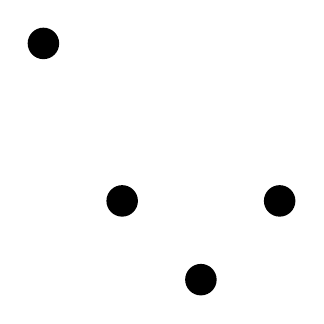
\begin{tikzpicture}
  \draw (0,0) pic {my circle=2mm};
  \draw (1,-2) pic {my circle=2mm};
  \draw (2,-3)  pic {my circle=2mm};
  \draw (3,-2)  pic {my circle=2mm};
\end{tikzpicture}}}

\newcommand{\majOne}{
\resizebox{5mm}{!}{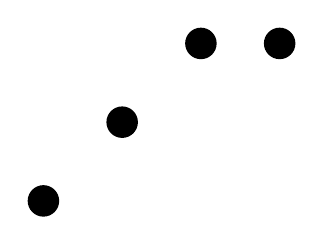
\begin{tikzpicture}
  \draw (0,-2) pic {my circle=2mm};
  \draw (1,-1) pic {my circle=2mm};
  \draw (2,0) pic {my circle=2mm};
  \draw (3,0) pic {my circle=2mm};
\end{tikzpicture}}}

\newcommand{\majFive}{
\resizebox{5mm}{!}{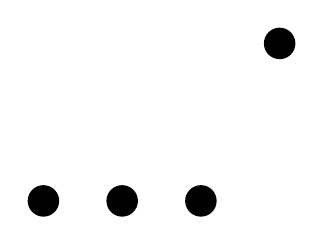
\begin{tikzpicture}
  \draw (0,-2) pic {my circle=2mm};
  \draw (1,-2) pic {my circle=2mm};
  \draw (2,-2) pic {my circle=2mm};
  \draw (3,0) pic {my circle=2mm};
\end{tikzpicture}}}

\newcommand{\majFiveB}{
\resizebox{5mm}{!}{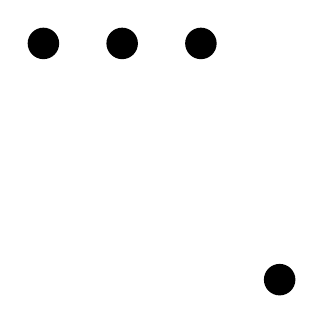
\begin{tikzpicture}
  \draw (0,0) pic {my circle=2mm};
  \draw (1,0) pic {my circle=2mm};
  \draw (2,0) pic {my circle=2mm};
  \draw (3,-3) pic {my circle=2mm};
\end{tikzpicture}}}

\newcommand{\majThree}{
\resizebox{5mm}{!}{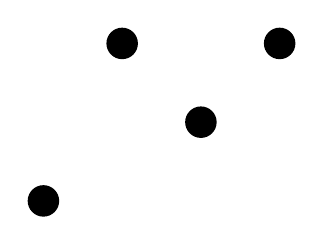
\begin{tikzpicture}
  \draw (0,-3) pic {my circle=2mm};
  \draw (1,-1) pic {my circle=2mm};
  \draw (2,-2) pic {my circle=2mm};
  \draw (3,-1) pic {my circle=2mm};
\end{tikzpicture}}}

%%



\newcommand{\minOne}{
\resizebox{5mm}{!}{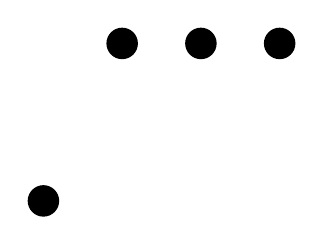
\begin{tikzpicture}
  \draw (0,-2) pic {my circle=2mm};
  \draw (1,0) pic {my circle=2mm};
  \draw (2,0)  pic {my circle=2mm};
  \draw (3,0)  pic {my circle=2mm};
\end{tikzpicture}}}

\newcommand{\minFive}{
\resizebox{5mm}{!}{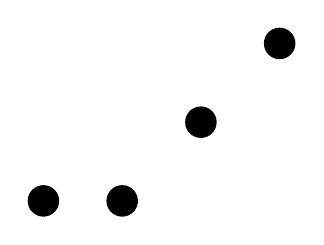
\begin{tikzpicture}
  \draw (0,-2) pic {my circle=2mm};
  \draw (1,-2) pic {my circle=2mm};
  \draw (2,-1) pic {my circle=2mm};
  \draw (3,0)  pic {my circle=2mm};
\end{tikzpicture}}}

\newcommand{\minThree}{
\resizebox{5mm}{!}{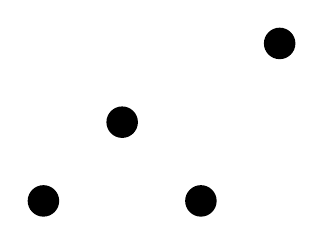
\begin{tikzpicture}
  \draw (0,-3) pic {my circle=2mm};
  \draw (1,-2) pic {my circle=2mm};
  \draw (2,-3) pic {my circle=2mm};
  \draw (3,-1) pic {my circle=2mm};
\end{tikzpicture}}}

%%

\newcommand{\deltaFive}{
\resizebox{5mm}{!}{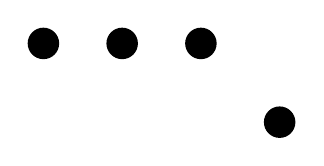
\begin{tikzpicture}
  \draw (0,0) pic {my circle=2mm};
  \draw (1,0) pic {my circle=2mm};
  \draw (2,0)  pic {my circle=2mm};
  \draw (3,-1)  pic {my circle=2mm};
\end{tikzpicture}}}

\newcommand{\deltaOne}{
\resizebox{5mm}{!}{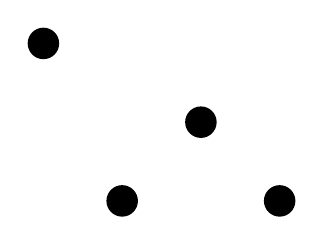
\begin{tikzpicture}
  \draw (0,0) pic {my circle=2mm};
  \draw (1,-2) pic {my circle=2mm};
  \draw (2,-1)  pic {my circle=2mm};
  \draw (3,-2)  pic {my circle=2mm};
\end{tikzpicture}}}

\newcommand{\deltaSeven}{
\resizebox{5mm}{!}{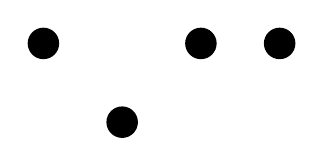
\begin{tikzpicture}
  \draw (0,0) pic {my circle=2mm};
  \draw (1,-1) pic {my circle=2mm};
  \draw (2,-0) pic {my circle=2mm};
  \draw (3,0)  pic {my circle=2mm};
\end{tikzpicture}}}

\newcommand{\deltaThree}{
\resizebox{5mm}{!}{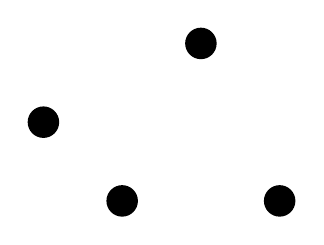
\begin{tikzpicture}
  \draw (0,-1) pic {my circle=2mm};
  \draw (1,-2) pic {my circle=2mm};
  \draw (2, 0) pic {my circle=2mm};
  \draw (3,-2) pic {my circle=2mm};
\end{tikzpicture}}}

\newcommand{\deltaStrange}{
\resizebox{5mm}{!}{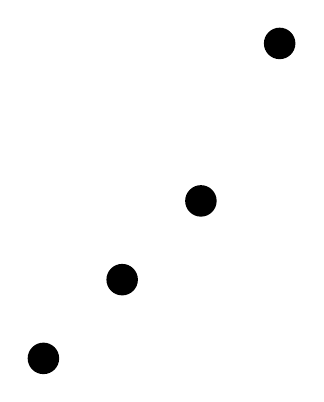
\begin{tikzpicture}
  \draw (0,-2) pic {my circle=2mm};
  \draw (1,-1) pic {my circle=2mm};
  \draw (2, 0) pic {my circle=2mm};
  \draw (3, 2) pic {my circle=2mm};
\end{tikzpicture}}}

\begin{document}

{\Large \book \textbf{Chords for Chicago Tuning}}

\bigskip

\begin{tabular}{lcccccc}
  \rotatebox{45}{Fret} & \rotatebox{45}{Bass} &  \rotatebox{45}{Maj1513} &\rotatebox{45}{Maj1351} & \rotatebox{45}{Maj5135} & \rotatebox{45}{Maj5131} & \rotatebox{45}{Maj3513} \\
     &                 & \majOneA         & \majOne           & \majFive        & \majFiveB       &\majThree               \\  
  0  & \writechord{C}  & \writechord{C}   & --                & --              & \writechord{F}  &\writechord{Bb}\\
  1  & \writechord{C#} & --               & --                & --              & \writechord{F#} &\writechord{B} \\
  2  & \writechord{D}  & --               & \writechord{D}    & \writechord{G}  & \writechord{G}  &\writechord{C} \\
  3  & \writechord{Eb} & --               & \writechord{Eb}   & \writechord{G#} & \writechord{G#} &\writechord{C#}\\
  4  & \writechord{E}  & --               & \writechord{E}    & \writechord{A}  & \writechord{A}  &\writechord{D} \\
  5  & \writechord{F}  & \writechord{F}   & \writechord{F}    & \writechord{Bb} & \writechord{Bb} &\writechord{Eb}\\
  6  & \writechord{F#} & \writechord{F#}  & \writechord{F#}   & \writechord{B}  & \writechord{B}  &\writechord{E}\\
  7  & \writechord{G}  & \writechord{G}   & \writechord{G}    & \writechord{C}  & \writechord{C}  &\writechord{F}  \\
  8  & \writechord{G#} & \writechord{G#}  & \writechord{G#}   & \writechord{C#} & \writechord{C#} &\writechord{F#} \\
  9  & \writechord{A}  & \writechord{A}   & \writechord{A}    & \writechord{D}  & \writechord{D}  &\writechord{G}  \\
  10 & \writechord{Bb} & \writechord{Bb}  & \writechord{Bb}   & \writechord{Eb} & \writechord{Eb} &\writechord{G#} \\
  11 & \writechord{B}  & \writechord{B}   & \writechord{B}    & \writechord{E}  & \writechord{E}  &\writechord{A}  \\
  12 & \writechord{C}  & \writechord{C}   & \writechord{C}    & \writechord{F}  & \writechord{F}  &\writechord{Bb}\\
\end{tabular}                               
\begin{tabular}{ccc}
 \rotatebox{45}{Min1351} & \rotatebox{45}{Min5135} & \rotatebox{45}{Min3513} \\
 \minOne           & \minFive        & \minThree               \\  
 --              & --              & --              \\
 --              & --              & --              \\
 \writechord{D}  & \writechord{G}  & \writechord{B}  \\
 \writechord{Eb} & \writechord{G#} & \writechord{C}  \\
 \writechord{E}  & \writechord{A}  & \writechord{C#} \\
 \writechord{F}  & \writechord{Bb} & \writechord{D}  \\
 \writechord{F#} & \writechord{B}  & \writechord{Eb} \\
 \writechord{G}  & \writechord{C}  & \writechord{F}  \\
 \writechord{G#} & \writechord{C#} & \writechord{F#} \\
 \writechord{A}  & \writechord{D}  & \writechord{G}  \\
 \writechord{Bb} & \writechord{Eb} & \writechord{G#} \\
 \writechord{B}  & \writechord{E}  & \writechord{A}  \\
 \writechord{C}  & \writechord{F}  & \writechord{Bb} \\
\end{tabular}
\begin{tabular}{ccccc}
 \rotatebox{45}{$\Delta$5137}& \rotatebox{45}{$\Delta$1573} & \rotatebox{45}{$\Delta$7351} & \rotatebox{45}{$\Delta$3715} & \rotatebox{45}{$\Delta$1537}\\
 \deltaFive      & \deltaOne       & \deltaSeven        & \deltaThree & \deltaStrange \\  
 \writechord{F}  & \writechord{C}  & --              & --              & --             \\
 \writechord{F#} & \writechord{C#} & \writechord{Eb} & \writechord{A}  & -- \\
 \writechord{G}  & \writechord{D}  & \writechord{F}  & \writechord{Bb} & --\\
 \writechord{G#} & \writechord{Eb} & \writechord{F#} & \writechord{B}  & -- \\
 \writechord{A}  & \writechord{E}  & \writechord{G}  & \writechord{C}  & \writechord{E} \\
 \writechord{Bb} & \writechord{F}  & \writechord{G#} & \writechord{C#} & -- \\
 \writechord{B}  & \writechord{F#} & \writechord{A}  & \writechord{D}  & -- \\
 \writechord{C}  & \writechord{G}  & \writechord{Bb} & \writechord{Eb} & \writechord{G}\\
 \writechord{C#} & \writechord{G#} & \writechord{B}  & \writechord{E}  & \writechord{G#} \\
 \writechord{D}  & \writechord{A}  & \writechord{C}  & \writechord{F}  & \writechord{A} \\
 \writechord{Eb} & \writechord{Bb} & \writechord{C#} & \writechord{F#} & \writechord{Bb}\\
 \writechord{E}  & \writechord{B}  & \writechord{D}  & \writechord{G}  & \writechord{B} \\
 \writechord{F}  & \writechord{C}  & \writechord{Eb} & \writechord{G#} & \writechord{C}\\
\end{tabular}

\clearpage

\begin{song}[transpose=+7]{title={Chords for Chicago Tuning [G]}, key=C}
\begin{tabular}{lcccccc}
  \rotatebox{45}{Fret} & \rotatebox{45}{Bass} &  \rotatebox{45}{Maj1513} &\rotatebox{45}{Maj1351} & \rotatebox{45}{Maj5135} & \rotatebox{45}{Maj5131} & \rotatebox{45}{Maj3513} \\
     &                 & \majOneA         & \majOne           & \majFive        & \majFiveB       &\majThree               \\  
  0  & \writechord{C}  & \writechord{C}   & --                & --              & \writechord{F}  &\writechord{Bb}\\
  1  & \writechord{C#} & --               & --                & --              & \writechord{F#} &\writechord{B} \\
  2  & \writechord{D}  & --               & \writechord{D}    & \writechord{G}  & \writechord{G}  &\writechord{C} \\
  3  & \writechord{Eb} & --               & \writechord{Eb}   & \writechord{G#} & \writechord{G#} &\writechord{C#}\\
  4  & \writechord{E}  & --               & \writechord{E}    & \writechord{A}  & \writechord{A}  &\writechord{D} \\
  5  & \writechord{F}  & \writechord{F}   & \writechord{F}    & \writechord{Bb} & \writechord{Bb} &\writechord{Eb}\\
  6  & \writechord{F#} & \writechord{F#}  & \writechord{F#}   & \writechord{B}  & \writechord{B}  &\writechord{E}\\
  7  & \writechord{G}  & \writechord{G}   & \writechord{G}    & \writechord{C}  & \writechord{C}  &\writechord{F}  \\
  8  & \writechord{G#} & \writechord{G#}  & \writechord{G#}   & \writechord{C#} & \writechord{C#} &\writechord{F#} \\
  9  & \writechord{A}  & \writechord{A}   & \writechord{A}    & \writechord{D}  & \writechord{D}  &\writechord{G}  \\
  10 & \writechord{Bb} & \writechord{Bb}  & \writechord{Bb}   & \writechord{Eb} & \writechord{Eb} &\writechord{G#} \\
  11 & \writechord{B}  & \writechord{B}   & \writechord{B}    & \writechord{E}  & \writechord{E}  &\writechord{A}  \\
  12 & \writechord{C}  & \writechord{C}   & \writechord{C}    & \writechord{F}  & \writechord{F}  &\writechord{Bb}\\
\end{tabular}                               
\begin{tabular}{ccc}
 \rotatebox{45}{Min1351} & \rotatebox{45}{Min5135} & \rotatebox{45}{Min3513} \\
 \minOne           & \minFive        & \minThree               \\  
 --              & --              & --              \\
 --              & --              & --              \\
 \writechord{D}  & \writechord{G}  & \writechord{B}  \\
 \writechord{Eb} & \writechord{G#} & \writechord{C}  \\
 \writechord{E}  & \writechord{A}  & \writechord{C#} \\
 \writechord{F}  & \writechord{Bb} & \writechord{D}  \\
 \writechord{F#} & \writechord{B}  & \writechord{Eb} \\
 \writechord{G}  & \writechord{C}  & \writechord{F}  \\
 \writechord{G#} & \writechord{C#} & \writechord{F#} \\
 \writechord{A}  & \writechord{D}  & \writechord{G}  \\
 \writechord{Bb} & \writechord{Eb} & \writechord{G#} \\
 \writechord{B}  & \writechord{E}  & \writechord{A}  \\
 \writechord{C}  & \writechord{F}  & \writechord{Bb} \\
\end{tabular}
\begin{tabular}{ccccc}
 \rotatebox{45}{$\Delta$5137}& \rotatebox{45}{$\Delta$1573} & \rotatebox{45}{$\Delta$7351} & \rotatebox{45}{$\Delta$3715} & \rotatebox{45}{$\Delta$1537}\\
 \deltaFive      & \deltaOne       & \deltaSeven        & \deltaThree & \deltaStrange \\  
 \writechord{F}  & \writechord{C}  & --              & --              & --             \\
 \writechord{F#} & \writechord{C#} & \writechord{Eb} & \writechord{A}  & -- \\
 \writechord{G}  & \writechord{D}  & \writechord{F}  & \writechord{Bb} & --\\
 \writechord{G#} & \writechord{Eb} & \writechord{F#} & \writechord{B}  & -- \\
 \writechord{A}  & \writechord{E}  & \writechord{G}  & \writechord{C}  & \writechord{E} \\
 \writechord{Bb} & \writechord{F}  & \writechord{G#} & \writechord{C#} & -- \\
 \writechord{B}  & \writechord{F#} & \writechord{A}  & \writechord{D}  & -- \\
 \writechord{C}  & \writechord{G}  & \writechord{Bb} & \writechord{Eb} & \writechord{G}\\
 \writechord{C#} & \writechord{G#} & \writechord{B}  & \writechord{E}  & \writechord{G#} \\
 \writechord{D}  & \writechord{A}  & \writechord{C}  & \writechord{F}  & \writechord{A} \\
 \writechord{Eb} & \writechord{Bb} & \writechord{C#} & \writechord{F#} & \writechord{Bb}\\
 \writechord{E}  & \writechord{B}  & \writechord{D}  & \writechord{G}  & \writechord{B} \\
 \writechord{F}  & \writechord{C}  & \writechord{Eb} & \writechord{G#} & \writechord{C}\\
\end{tabular}
\end{song}

\end{document}
